\documentclass[tikz,border=12pt]{standalone}
\usepackage{tikz}
\usepackage{xcolor}
\usepackage{amsmath}
\usetikzlibrary{shapes.geometric,positioning,calc,fit,backgrounds}

%% ── Phase colours (consistent with OODA diagram in CH1) ──────────────────
\definecolor{obsblue}{RGB}{219,234,254}      % observe  – light blue
\definecolor{origreen}{RGB}{220,252,231}     % orient   – light green
\definecolor{decyellow}{RGB}{254,249,195}    % decide   – light yellow
\definecolor{actpink}{RGB}{252,231,243}      % act      – light pink
\definecolor{patgray}{RGB}{241,245,249}      % patient profile
\definecolor{outorange}{RGB}{255,231,180}     % outcome box – light orange
\definecolor{arrowgray}{RGB}{107,114,128}

\tikzset{
  phasebox/.style={
    rectangle, rounded corners=4pt,
    minimum width=4.3cm, minimum height=8.6cm,
    text width=3.8cm, align=left,
    inner sep=7pt, font=\fontsize{7.4}{9.2}\selectfont
  },
  phaselabel/.style={
    font=\fontsize{8}{10}\selectfont\bfseries,
    text width=4.3cm, align=center
  },
  topbox/.style={
    rectangle, rounded corners=4pt,
    minimum width=17.8cm, text width=17.2cm,
    align=left, inner sep=9pt,
    font=\fontsize{7.8}{10}\selectfont
  },
  botbox/.style={
    rectangle, rounded corners=4pt,
    minimum width=17.8cm, text width=17.2cm,
    align=left, inner sep=9pt,
    font=\fontsize{7.8}{10}\selectfont
  },
  bullet/.style={font=\fontsize{7.4}{9.2}\selectfont},
}

\begin{document}
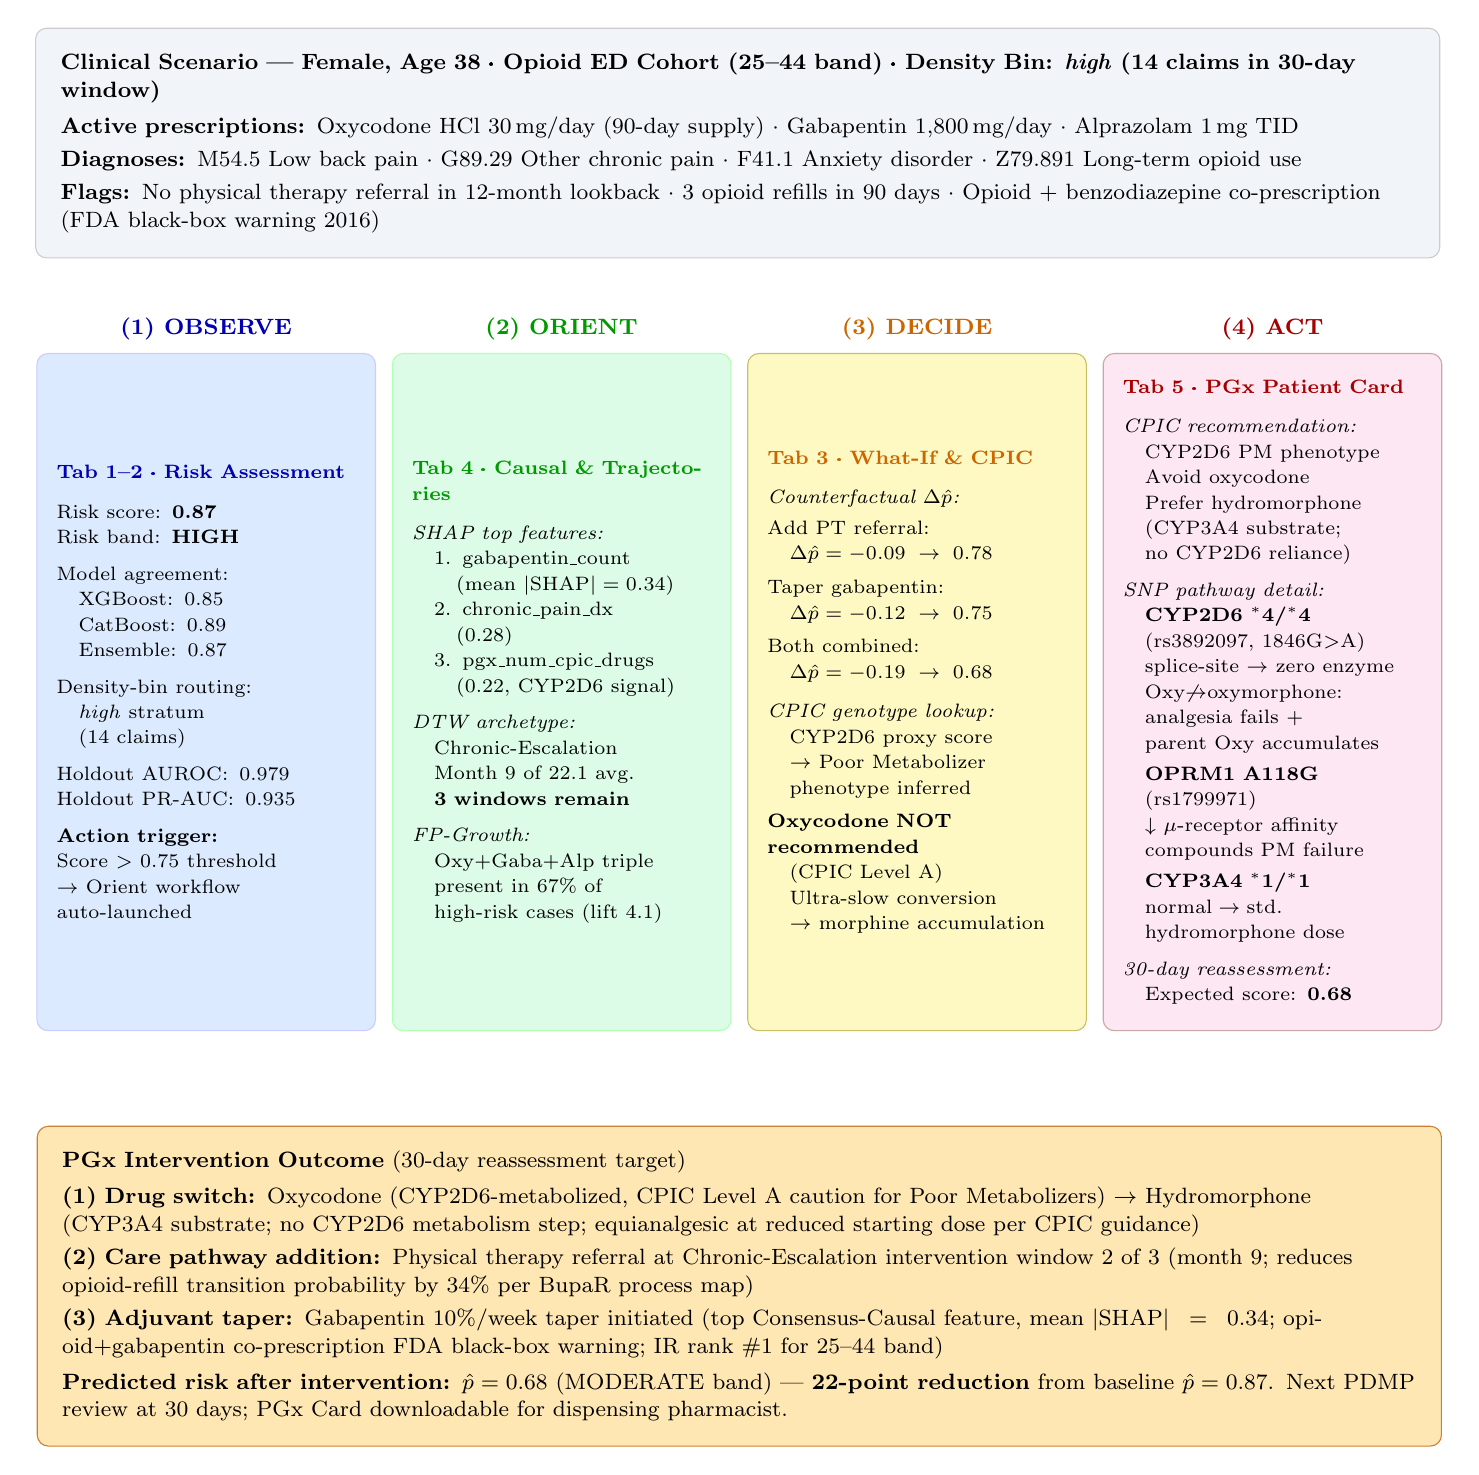
\begin{tikzpicture}

%% ── Patient profile (top) ────────────────────────────────────────────────
\node[topbox, fill=patgray, draw=gray!40] (patient) at (0,0) {%
  \textbf{Clinical Scenario — Female, Age~38 · Opioid ED Cohort (25--44 band) · Density Bin: \textit{high} (14 claims in 30-day window)}\\[3pt]
  \textbf{Active prescriptions:}\enspace
    Oxycodone HCl 30\,mg/day (90-day supply) $\cdot$
    Gabapentin 1{,}800\,mg/day $\cdot$
    Alprazolam 1\,mg TID\\[2pt]
  \textbf{Diagnoses:}\enspace
    M54.5 Low back pain $\cdot$
    G89.29 Other chronic pain $\cdot$
    F41.1 Anxiety disorder $\cdot$
    Z79.891 Long-term opioid use\\[2pt]
  \textbf{Flags:}\enspace
    No physical therapy referral in 12-month lookback $\cdot$
    3 opioid refills in 90 days $\cdot$
    Opioid + benzodiazepine co-prescription (FDA black-box warning 2016)
};

%% ── Phase boxes ──────────────────────────────────────────────────────────
\node[phasebox, fill=obsblue, draw=blue!20,
      below=1.2cm of patient, xshift=-6.75cm] (obs) {%
  \textbf{\color{blue!70!black}Tab~1--2 · Risk Assessment}\\[5pt]
  Risk score:\enspace\textbf{0.87}\\
  Risk band:\enspace\textbf{HIGH}\\[4pt]
  Model agreement:\\
  \quad XGBoost:\enspace 0.85\\
  \quad CatBoost:\enspace 0.89\\
  \quad Ensemble:\enspace 0.87\\[4pt]
  Density-bin routing:\\
  \quad \textit{high} stratum\\
  \quad (14 claims)\\[4pt]
  Holdout AUROC:\enspace 0.979\\
  Holdout PR-AUC:\enspace 0.935\\[4pt]
  \textbf{Action trigger:}\\
  Score $>$ 0.75 threshold\\
  $\rightarrow$ Orient workflow\\
  auto-launched
};

\node[phasebox, fill=origreen, draw=green!30,
      right=0.2cm of obs] (ori) {%
  \textbf{\color{green!60!black}Tab~4 · Causal \& Trajectories}\\[5pt]
  \textit{SHAP top features:}\\
  \quad 1.\enspace gabapentin\_count\\
  \qquad (mean $|\text{SHAP}|=0.34$)\\
  \quad 2.\enspace chronic\_pain\_dx\\
  \qquad (0.28)\\
  \quad 3.\enspace pgx\_num\_cpic\_drugs\\
  \qquad (0.22, CYP2D6 signal)\\[4pt]
  \textit{DTW archetype:}\\
  \quad Chronic-Escalation\\
  \quad Month~9 of 22.1 avg.\\
  \quad \textbf{3 windows remain}\\[4pt]
  \textit{FP-Growth:}\\
  \quad Oxy+Gaba+Alp triple\\
  \quad present in 67\% of\\
  \quad high-risk cases (lift 4.1)
};

\node[phasebox, fill=decyellow, draw=yellow!50!gray,
      right=0.2cm of ori] (dec) {%
  \textbf{\color{orange!80!black}Tab~3 · What-If \& CPIC}\\[5pt]
  \textit{Counterfactual $\Delta\hat{p}$:}\\[2pt]
  Add PT referral:\\
  \quad $\Delta\hat{p}=-0.09\;\to\;0.78$\\[3pt]
  Taper gabapentin:\\
  \quad $\Delta\hat{p}=-0.12\;\to\;0.75$\\[3pt]
  Both combined:\\
  \quad $\Delta\hat{p}=-0.19\;\to\;0.68$\\[5pt]
  \textit{CPIC genotype lookup:}\\
  \quad CYP2D6 proxy score\\
  \quad $\rightarrow$ Poor Metabolizer\\
  \quad phenotype inferred\\[3pt]
  \textbf{Oxycodone NOT}\\
  \textbf{recommended}\\
  \quad (CPIC Level~A)\\
  \quad Ultra-slow conversion\\
  \quad $\rightarrow$ morphine accumulation
};

\node[phasebox, fill=actpink, draw=pink!60!gray,
      right=0.2cm of dec] (act) {%
  \textbf{\color{red!65!black}Tab~5 · PGx Patient Card}\\[5pt]
  \textit{CPIC recommendation:}\\
  \quad CYP2D6 PM phenotype\\
  \quad Avoid oxycodone\\
  \quad Prefer hydromorphone\\
  \quad (CYP3A4 substrate;\\
  \quad no CYP2D6 reliance)\\[4pt]
  \textit{SNP pathway detail:}\\
  \quad \textbf{CYP2D6 ${}^{*}$4/${}^{*}$4}\\  \quad (rs3892097, 1846G$>$A)\\
  \quad splice-site $\to$ zero enzyme\\
  \quad Oxy$\not\to$oxymorphone:\\
  \quad analgesia fails $+$\\
  \quad parent Oxy accumulates\\[2pt]
  \quad \textbf{OPRM1 A118G}\\
  \quad (rs1799971)\\
  \quad $\downarrow$ $\mu$-receptor affinity\\
  \quad compounds PM failure\\[2pt]
  \quad \textbf{CYP3A4 ${}^{*}$1/${}^{*}$1}\\
  \quad normal\;$\to$\;std.\\
  \quad hydromorphone dose\\[4pt]
  \textit{30-day reassessment:}\\
  \quad Expected score:\enspace\textbf{0.68}
};

%% ── Phase title labels above each box ────────────────────────────────────
\node[phaselabel, above=1pt of obs.north]
  {\textcolor{blue!70!black}{(1) OBSERVE}};
\node[phaselabel, above=1pt of ori.north]
  {\textcolor{green!60!black}{(2) ORIENT}};
\node[phaselabel, above=1pt of dec.north]
  {\textcolor{orange!80!black}{(3) DECIDE}};
\node[phaselabel, above=1pt of act.north]
  {\textcolor{red!65!black}{(4) ACT}};

%% ── Outcome box (bottom, centered via phase midpoint) ─────────────────────────
\coordinate (phasemid) at ($(obs.south)!0.5!(act.south)$);
\node[botbox, fill=outorange, draw=orange!60!gray,
      below=1.2cm of phasemid] (outcome) {%
  \textbf{PGx Intervention Outcome} (30-day reassessment target)\\[3pt]
  \textbf{(1) Drug switch:}\enspace
    Oxycodone (CYP2D6-metabolized, CPIC Level~A caution for Poor Metabolizers)
    $\rightarrow$ Hydromorphone (CYP3A4 substrate; no CYP2D6 metabolism step;
    equianalgesic at reduced starting dose per CPIC guidance)\\[2pt]
  \textbf{(2) Care pathway addition:}\enspace
    Physical therapy referral at Chronic-Escalation intervention window~2 of~3
    (month~9; reduces opioid-refill transition probability by 34\% per BupaR process map)\\[2pt]
  \textbf{(3) Adjuvant taper:}\enspace
    Gabapentin 10\%/week taper initiated
    (top Consensus-Causal feature, mean $|\text{SHAP}|=0.34$; opioid+gabapentin
    co-prescription FDA black-box warning; IR rank~\#1 for 25--44 band)\\[3pt]
  \textbf{Predicted risk after intervention:}\enspace
    $\hat{p}=0.68$ (MODERATE band) ---
    \textbf{22-point reduction} from baseline $\hat{p}=0.87$.
    Next PDMP review at 30~days; PGx Card downloadable for dispensing pharmacist.
};


\end{tikzpicture}
\end{document}
